
%************************************************
\section{Validation and Performance Evaluation}\label{ch:validation}
%************************************************

In this section, we will describe the deployment of three testing scenarios: a laptop, a Raspberry Pi 3, and an Omega2 IoT device with the Raspberry Pi 3 as the delegation server. We will measure and compare the results to determine if the proposed solution runs as expected and is feasible.

\subsection{Testbed description}

First, we shall describe the example Attribute Based Credential system in use. Then, the hardware we will use in our benchmarking.

\subsubsection{P2ABCE setting}

To test the correct execution of the \textit{IoT smart card}, we will use the ABC system from the tutorial in the P2ABCE Wiki\footnote{\url{https://github.com/p2abcengine/p2abcengine/wiki/}}. It is based on a soccer club, which wishes to issue VIP-tickets for a match. The VIP-member number in the ticket is inspectable for a lottery, ie. after the game, a random presentation token is inspected and the winning member is notified.

First go through the \textbf{setup} phase, where several artifacts are generated and distributed to the various P2ABCE entities. Then a ticket credential containing the following attributes is issued:

\begin{verbatim}
First name: John
Last name: Dow
Birthday: 1985-05-05Z
Member number: 23784638726
Matchday: 2013-08-07Z
\end{verbatim}

During \textbf{issuance}, a \textit{scope exclusive pseudonym} is established and the newly issued credential is bound to this pseudonym. This ensures that the ticket credential can not be used without the smart card.

Then \textbf{presentation} is performed, where a \textit{presentation policy} from the verifier specifies that the member number is inspectable and a predicate ensures that the matchday is in fact $2013-08-07Z$. This last part ensures that a ticket issued for another match can not be used.

\hfil

\subsubsection{Execution environment}

First we will execute the test in our development machine (laptop). After asserting that the services work as expected, we then run the test in a Raspberry Pi 3\footnote{\url{https://www.raspberrypi.org/products/raspberry-pi-3-model-b/}}, exactly like in the laptop. Finally, we will deploy the IoT smart card in an Omega2\footnote{\url{https://docs.onion.io/omega2-docs/omega2.html}} and the delegation services in the Raspberry Pi 3. After every test, we checked that the issuing and proving were successful, in case a cryptographic error appeared in the implementation.
A downside of using the Omega2 is the lack of hardware acceleration for cryptographic operations, unlike the MULTOS smart cards.



\paragraph{The network} In our third scenario, the Raspberry Pi 3 and the Omega2 will talk to each other over TCP. This implies possible network delays depending on the quality of the connection. The Raspberry Pi 3 is connected over Ethernet to a switch with WiFi access point. The Omega2 is connected over WiFi n to said AP. To ensure the delay wasn't significant, we measured 6000 APDU messages taken from previous executions, and the results show that the mean transmission time is less than half a millisecond per APDU. From our analysis of the tests we conclude that the network time is negligible compared to the rest of the computations.



\subsection{Results}

After 20 executions for each scenario (laptop, RPi3, Omega2+RPi3), we measure the time of each REST call executed against the User Service in the delegation server and take the means to compare each step of the testbed. Because during a call to the User Service, the server may contact the \textit{IoT Smart Card}, the difference in times between the second and third scenario will show the performance of our PoC.

It is worth noting that during the test, the measured use of the CPU showed that P2ABCE does not benefit of parallelization, therefore, it only uses one of the four cores in the laptop and Raspberry Pi 3.

\paragraph{The setup}\hfil

During the first step of our testbed the Omega2 doesn't intervene until the creation of the smart card, therefore, the times measured for each REST call in the second and third scenarios are practically identical.

\begin{figure}[bth]
	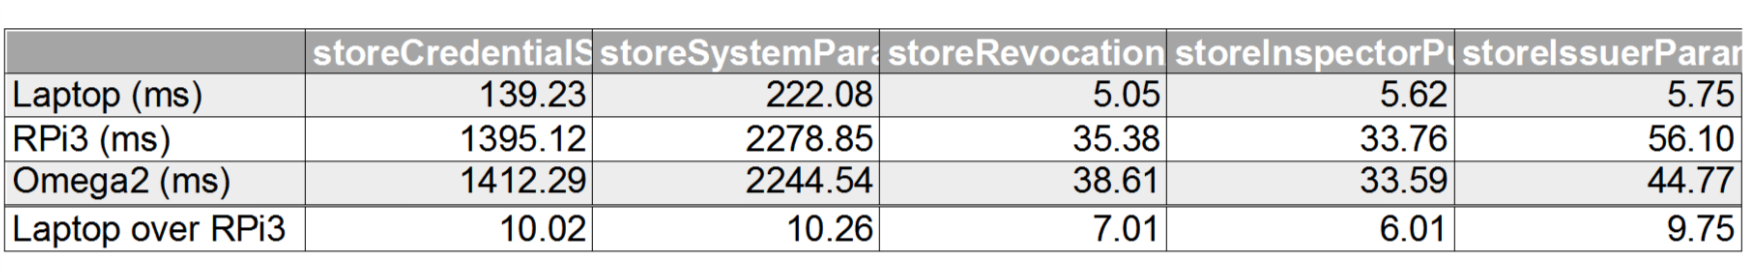
\includegraphics[width=\linewidth]{gfx/graphics/setuptable}
	\caption{Setup times (milliseconds) and relative speedup.}
	\label{fig:setup:graph}
\end{figure}

%\begin{figure}[bth]
%	\caption{Setup times (milliseconds). Comparison graph}
%	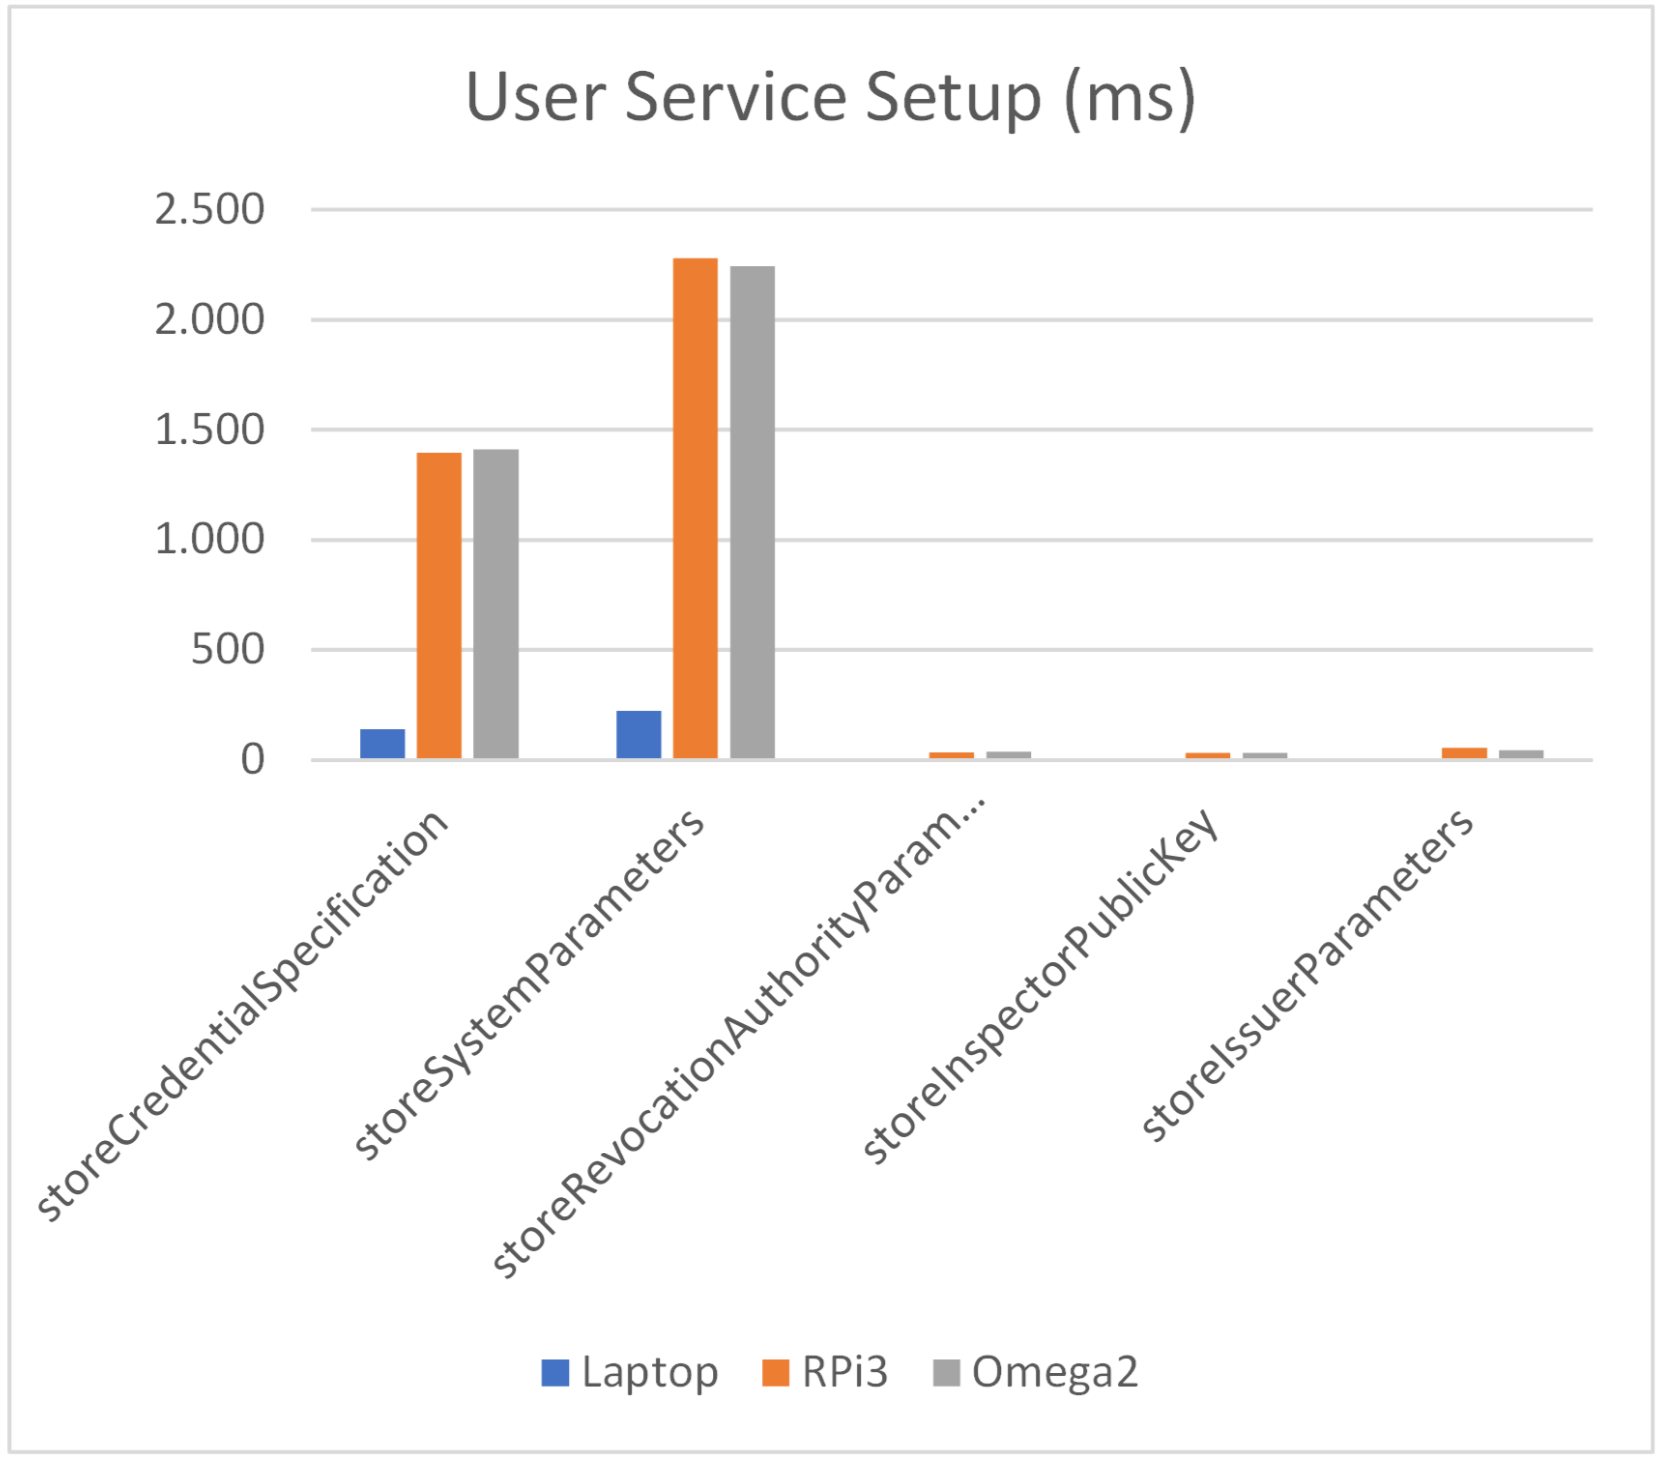
\includegraphics[width=0.8\linewidth]{gfx/graphics/setup}
%	\label{fig:setup:graph2}
%\end{figure}

As we can see in \autoref{fig:setup:graph}, the laptop is about ten times faster than Raspberry Pi 3, but considering that the highest time is less than two and a half seconds, and that the setup is done only once, this isn't a worrisome problem.

\paragraph{Creation of the smart card}\hfil

Here we create a \textit{SoftwareSmartcard} or a \textit{HardwareSmartcard}, pointing to the \textit{IoT Smart Card}, object that the User service will use in the following REST calls.

The REST method to create a \textit{SoftwareSmartcard} is $/createSmartcard$, and to create a \textit{HardwareSmartcard}, using the \textit{IoTsmartcardio} implementation, we use $/initIoTsmartcard$. This operation is done only once per device, and includes APDU Commands from the creation of the PIN and PUK of the smart card, to storing the system parameters from the previous setup step.

\begin{figure}[bth]
	\centerline{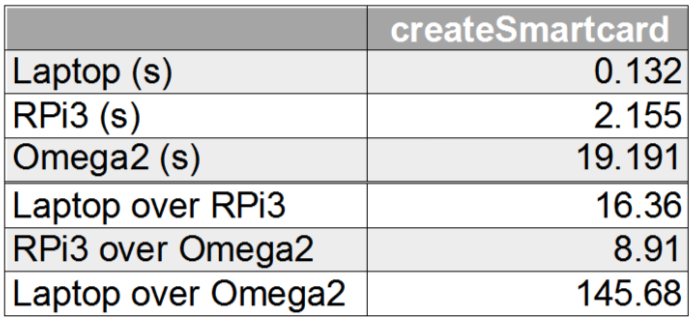
\includegraphics[width=0.4\linewidth]{gfx/graphics/createSCtable}}
	\caption{Create smart card times (seconds) and relative speedup.}
	\label{fig:createSmartCard:graph}
\end{figure}

%\begin{figure}[bth]
%	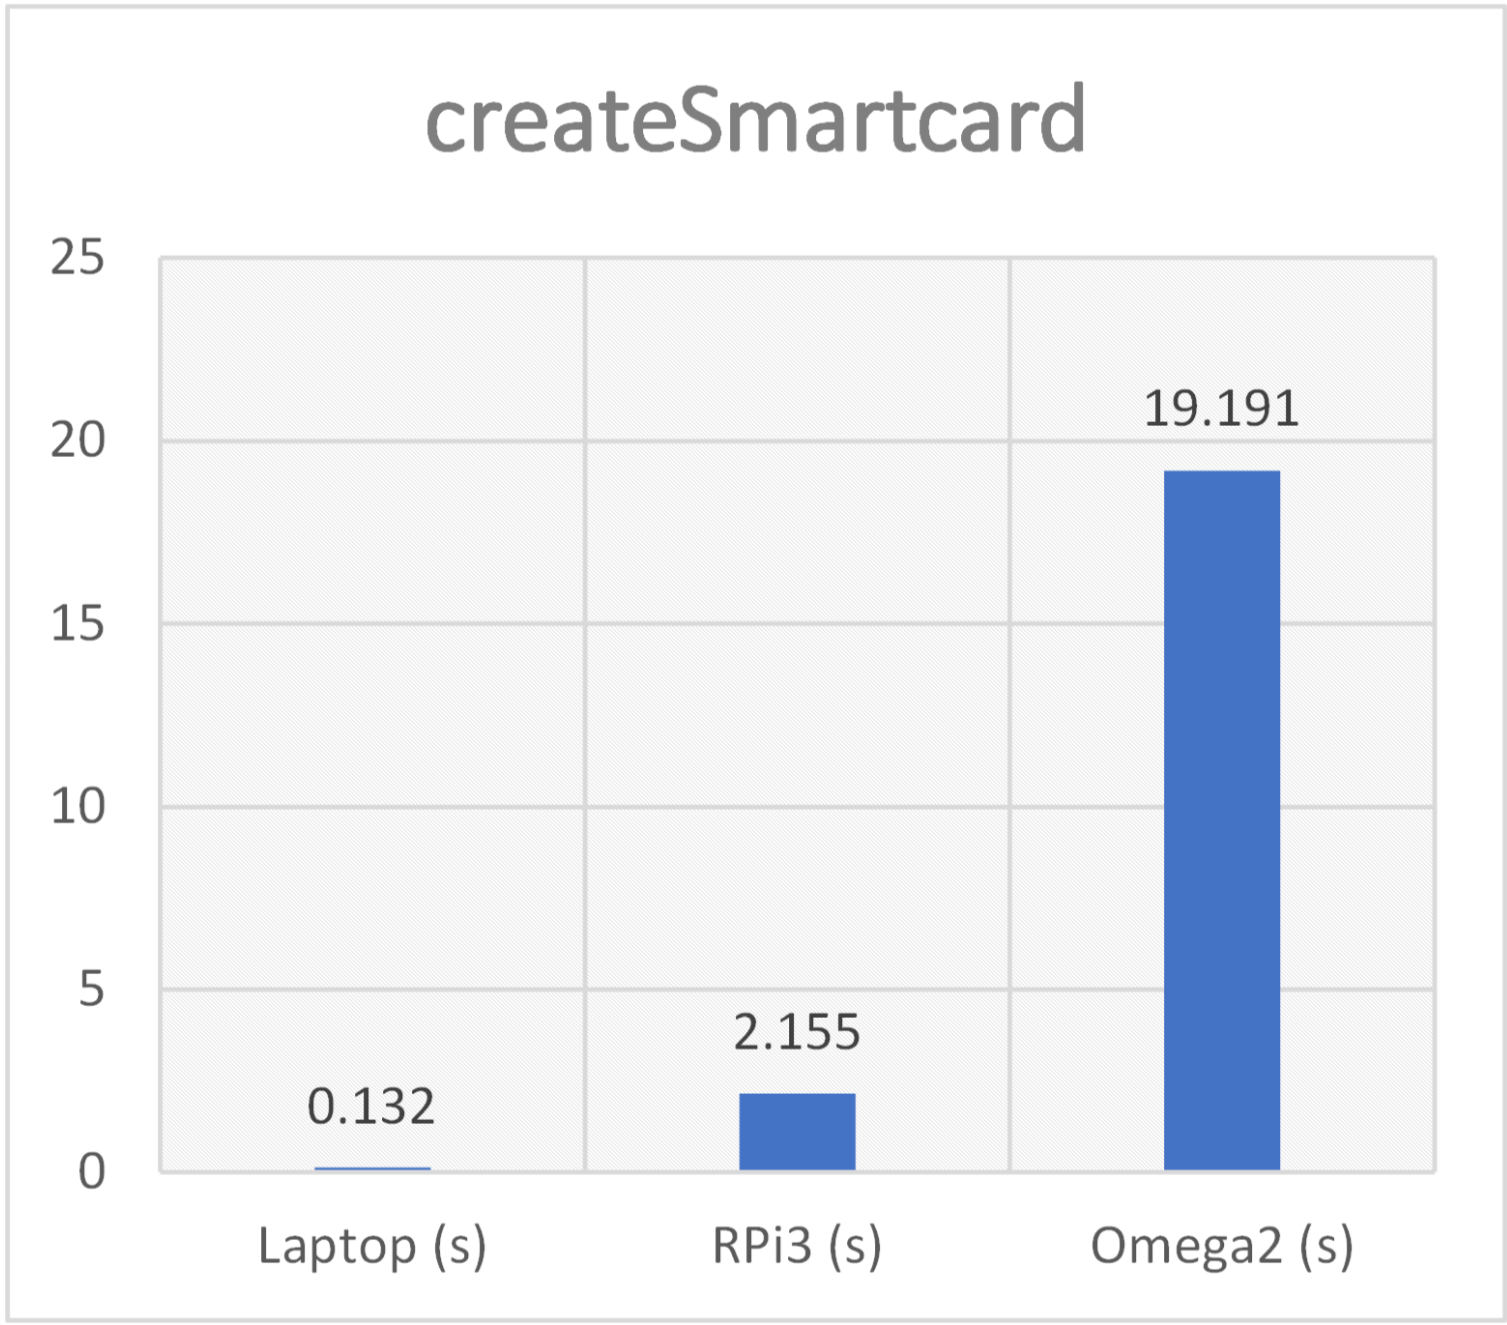
\includegraphics[width=0.8\linewidth]{gfx/graphics/createSC}
%	\caption{Create smart card times (seconds). Comparison graph}
%	\label{fig:createSmartCard:graph2}
%\end{figure}


From \autoref{fig:createSmartCard:graph} we see that the RPi3 is about 16 times slower than the laptop in the creation of the \textit{SoftwareSmartcard}, but almost 9 times faster than the setup of the smart card in the Omega2 using APDUs. This gives us that the laptop is 145 times faster than the combination of RPi3 and Omega2 in our IoT deployment.
But looking at the times, this process lasts up to 20 seconds, making it something feasible for a one time process.

This is the first interaction between the RPi3 and the IoT smart card running in the Omega2. To setup the smart card 30 APDU Commands, and their respective Responses, are exchanged, with a total of $1109$ bytes. From our network benchmark, using TCP sockets, the delay in the transmission is only around 15 and 20 ms, negligible, as we said, compared to the almost 20 seconds the operation lasts.


\paragraph{Issuance of the credential}\hfil

Our credential will have 5 attributes and key sizes of 1024 bits, as specified during the setup process.

The three delegation steps and the REST method called are:

\begin{itemize}
	\item First issuance protocol step:\\\texttt{/issuanceProtocolStep}
	\item Second issuance protocol step (end of first step for the User): \texttt{/issuanceProtocolStepUi}
	\item Third issuance protocol step (second step for the User): \texttt{/issuanceProtocolStep}
\end{itemize}

%\begin{center}
%	\begin{tabular}{l|l}
%		First issuance protocol step & $/issuanceProtocolStep$ \\
%		Second issuance protocol step  & $/issuanceProtocolStepUi$ \\
%		\textit{(end of first step for the User)} & \\
%		Third issuance protocol step & $/issuanceProtocolStep$ \\
%		\textit{(second step for the User)}  & \\
%	\end{tabular}
%\end{center}


%\begin{figure}[bth]
%	\begin{center}
%		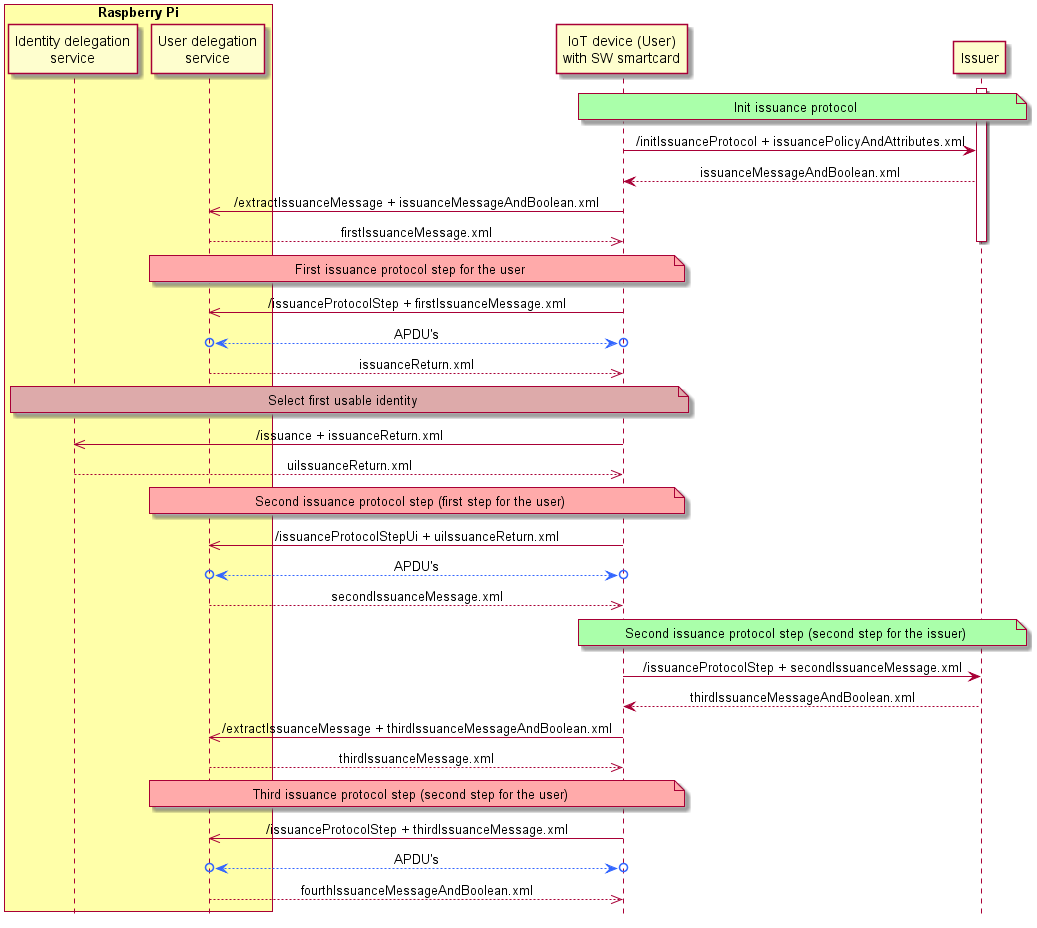
\includegraphics[width=\linewidth]{gfx/UML/IssuanceInteraction}
%	\end{center}
%	\caption{Issuance interaction.}
%	\label{fig:IssuanceInteraction}
%\end{figure}



As we can see, the three REST calls to the delegation User service involve communication with the smart card. There are 45 APDU Commands in total, $3197$ bytes exchanged, that would introduce a latency of 45ms in the network, negligible.


\begin{figure}[bth]
	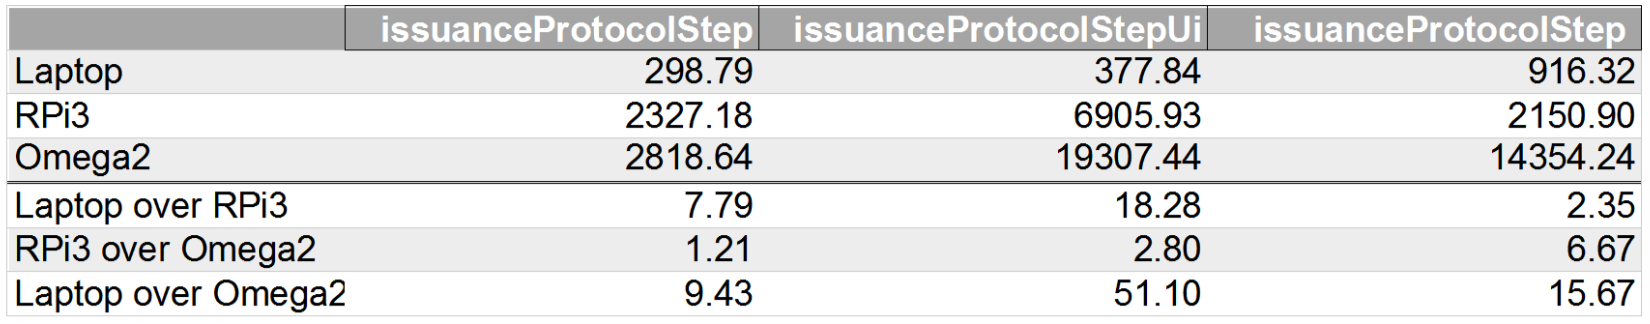
\includegraphics[width=\linewidth]{gfx/graphics/issuancetable}
	\caption{Issuance times (milliseconds) and relative speedup.}
	\label{fig:issuance:graph}
\end{figure}

%\begin{figure}[bth]
%	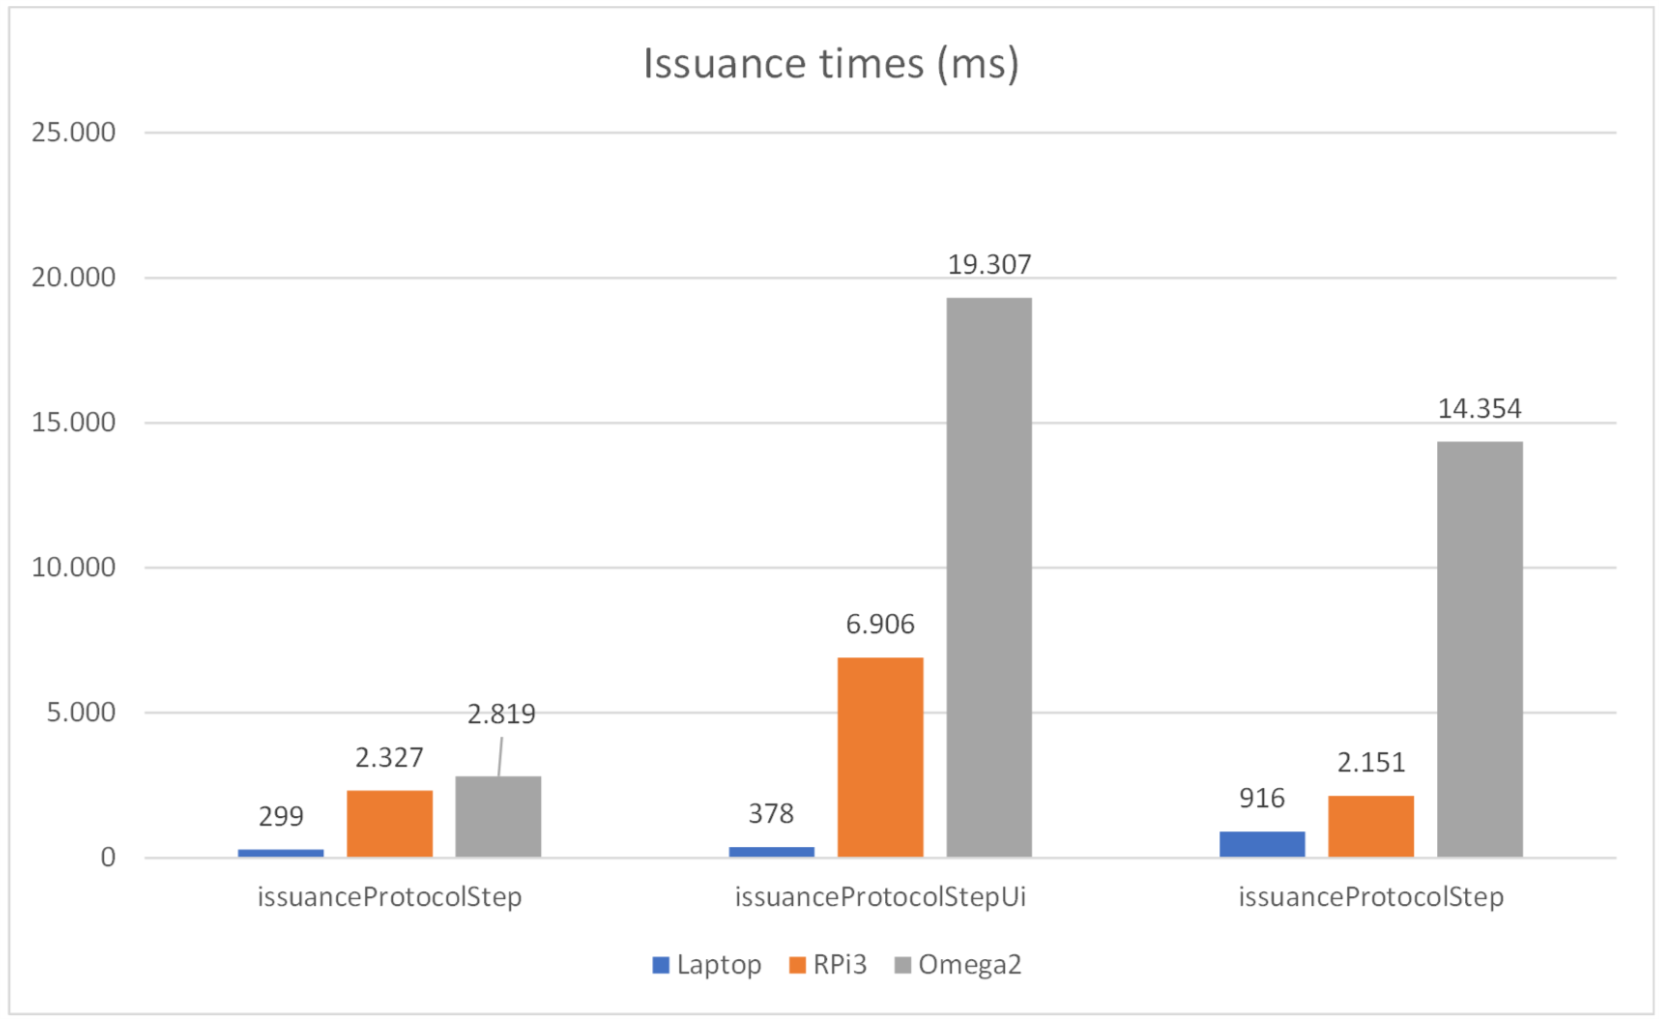
\includegraphics[width=\linewidth]{gfx/graphics/issuance}
%	\caption{Issuance times (milliseconds). Comparison graph}
%	\label{fig:issuance:graph2}
%\end{figure}

In \autoref{fig:issuance:graph} we have the times spent in each REST call. The laptop shows again to be many times faster than the other two scenarios, but the times are again feasible for an IoT environment.

Lets compare the Raspberry Pi 3 and the Omega2 scenarios. There is a correlation between the APDU Commands used in each step with the increment in time when using the \textit{IoT Smart Card}.
During the first REST call, only one APDU pair (Command and Response) was used, with $33$ bytes total, and times are almost identical. The second call needed $34$ APDUs, with $1623$ bytes, and the increase in time is around tree times slower than the RPi3 on its own. The third call used $20$ APDUs, $1541$ bytes, and makes the IoT scenario almost 7 times slower. 
The analysis shows where there are more cryptographic operations involving the Omega2, and because the amount of data exchanged is minimal, we can see the difference in processing power between Omega2 and Raspberry Pi 3.



\paragraph{Presentation token}\hfil

The final step of the test involves a Prove, or Presentation in P2ABCE, where the Verifier sends the User or Prover the Presentation Policy, and the User answers with the Presentation Token, without more steps. 
%In \autoref{fig:ProvingInteraction}, using the same colors as in the Issuance interaction, we can see the delegation messages done by the Omega2.

To ensure that all the process was successful, it's enough to check with the Verifier and the Inspector they accepted the prove or returned an error code. Of course, every execution measured in the test was successful, validating the PoC implementation.

%The APDU Commands and Responses pairs sent are $28$ in total, with $1939$ bytes, giving us about $27$ms of delay in the network transmission.



%\begin{figure}[bth]
%	\begin{center}
%		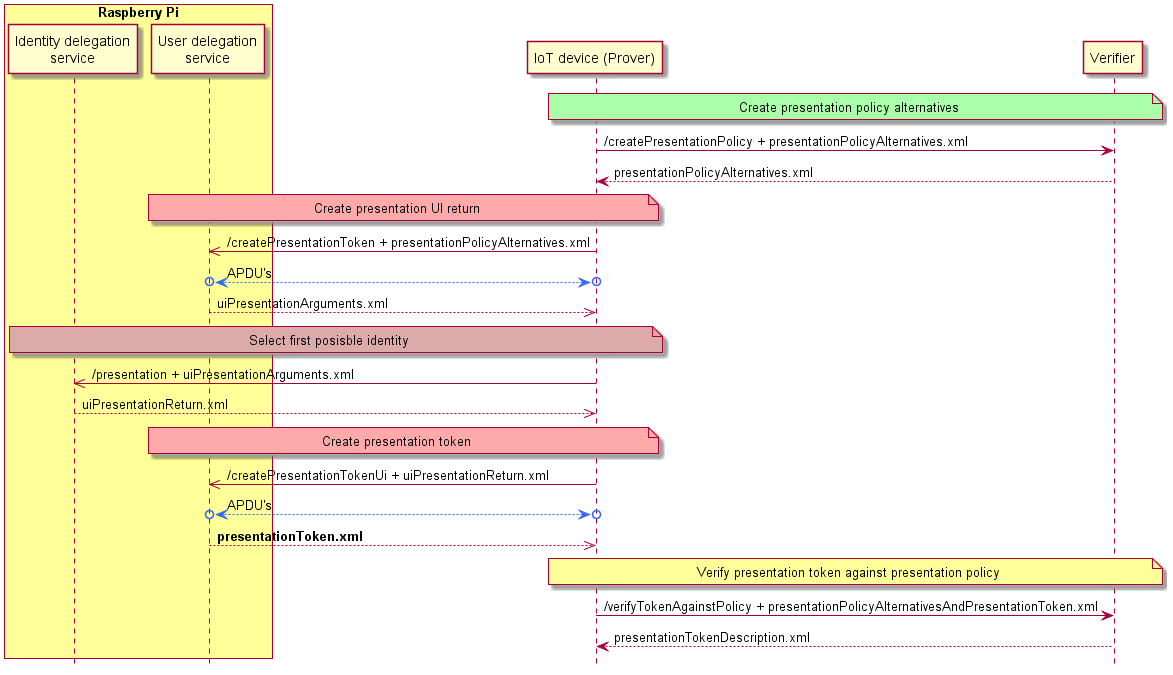
\includegraphics[width=\linewidth]{gfx/UML/ProvingInteraction}
%	\end{center}
%	\caption{Proving interaction.}
%	\label{fig:ProvingInteraction}
%\end{figure}



Again, as shown in \autoref{fig:proving:graph}, there is a correlation between the number of APDU Commands used, the work the IoT smart card must perform, and the time measured. The $20$ APDU Commands in the first call make the IoT deployment almost $8$ times slower than the Raspberry Pi 3; but with only $8$ APDU Commands, the second one is less than $1.5$ times slower.

%Nonetheless, it's significant the difference in performance between the laptop and the Raspberry Pi 3 in the last REST call, more than $40$ times slower, even using the \textit{SoftwareSmartcard} in the RPi3.


\begin{figure}[bth]
	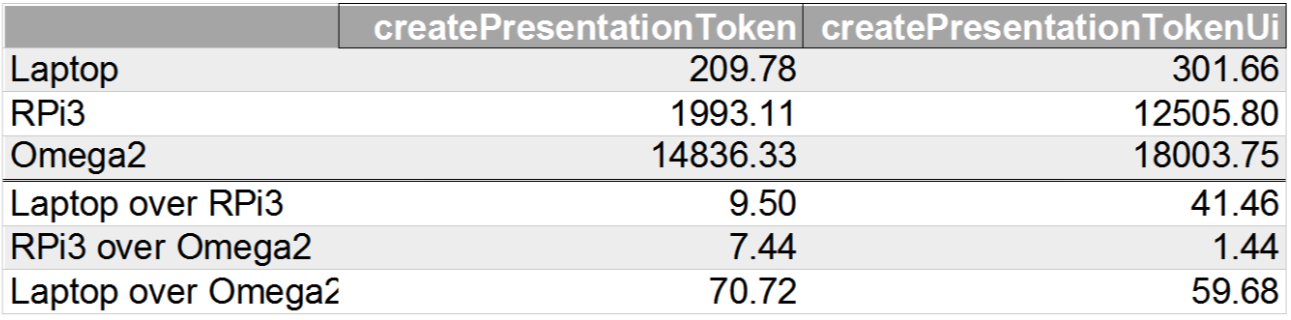
\includegraphics[width=.8\linewidth]{gfx/graphics/provingtable}
	\caption{Proving times (milliseconds) and relative speedup.}
	\label{fig:proving:graph}
\end{figure}

%\begin{figure}[bth]
%	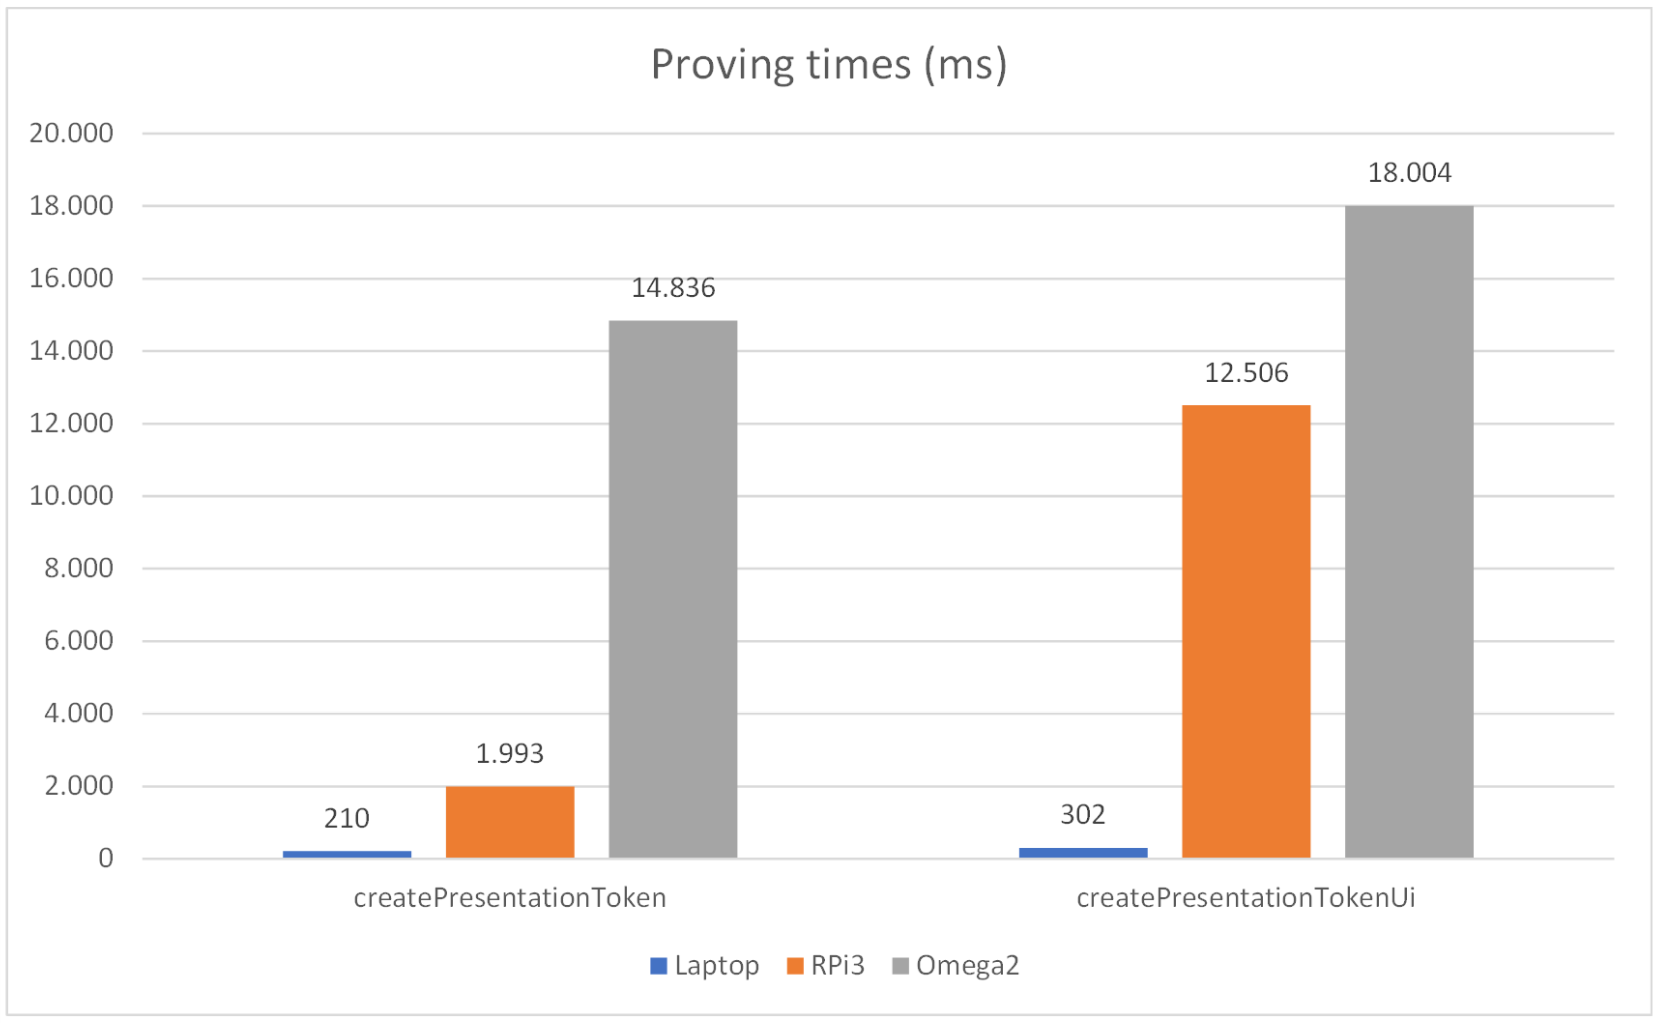
\includegraphics[width=\linewidth]{gfx/graphics/proving}
%	\caption{Proving times (milliseconds). Comparison graph}
%	\label{fig:proving:graph2}
%\end{figure}

Unlike the previous steps, the Presentation or Proving is done more than once, being the key feature of P2ABC ecosystem. The laptop performs a prove in less than one second, the RPi3 needs $15$ seconds, but our P2ABCE IoT deployment needs $15$ seconds for the first step, and $18$s for the second step, $33$ seconds total to generate a Presentation Token.




\hfil

\paragraph{Memory usage on the Omega2}\hfil

Using the tool \texttt{time -v} we can get a lot of useful information about a program, once it finishes. In our case, we measure the \textit{IoT Smart Card} binary running in the Omega 2, after the described testbed execution.

After another round of tests, the field in the \texttt{time} output named \texttt{Maximum resident set size (kbytes)} shows the maximum size of RAM used by the process since its launch. In our case, this involves the use of static memory for the \textit{global variables} of the smart card logic, and the dynamic memory used by the third party libraries, like GMPlib, OpenSSL and cJSON.

GMP and OpenSSL always allocate the data in their own ADT, what involves copying the arrays of bytes representing the big modular integers from the cryptographic operations. cJSON, used in the serialization of the smart card for storage, and debugging purposes, it stores a copy of every saved variable in the JSON tree structure, then creates a string with the JSON, that the user can then write to the save file.

Understanding the many bad uses of memory done in this PoC is important for future improvements and ports. A custom modular library using the same array of bytes that the smart card logic, an optimized binary serialization method, and many other improvements, are part of our future work.

With all that said, the mean of the maximum memory usage measured is $6569.6$ kbytes. Compared to the $64$MB of RAM available in the Omega2, our PoC could be executed in even more constrained devices.


\subsection{Validation conclusions}

Below \autoref{totaltime} sums up the time in seconds used in each step of the test for the Omega2 scenario.

The first step, \textit{System Setup} is done only once when the system is being deployed, and the \textit{IoT Smart Card Setup} only once per device.

Because a device can have more than one credential, the Issuance step is significant when we issue multiple credentials over the device's lifetime. We recall that our tests used a credential with five attributes and key sizes of 1024 bits.

Finally, the Proving step is expected to be the most commonly performed operation. The fact that it lasts over half a minute implies that we should not use this PoC for \textit{real-time} applications yet. Nevertheless, for many other IoT applications, the fact this operation can be performed multiple times per hour, presents an useful tool for privacy.


\begin{table}[!ht]
	\begin{center}
		\begin{tabular}{|r|r|r|r|}
			\hline
			System & IoT Smart  & Issue  & Prove Presen-\\
			Setup & Card Setup & credential & tation Policy\\ \hline
			3.77 s & 19.19 s & 36.48 s & 32.84 s \\ \hline
		\end{tabular}
	\end{center}
	\caption{Total time spent for each step in the Omega2+RPi3 scenario.}
	\label{totaltime}
\end{table}


